\documentclass[tikz,border=2pt]{standalone}
\usepackage{amsmath}
\usepackage{pgfplots}
\pgfplotsset{compat=1.18}
\usetikzlibrary{arrows.meta}
\begin{document}
% Discrete-time queue with L_0 = 2, arrivals 3,0,4,1,0 and capacity c_k = 2. Without service in the
% arrival period, d_k = min{L_{k-1}, c_k}: L = 2,3,1,4,3,1. With it, L_k = [L_{k-1}+a_k-c_k]^+: L = 2,3,1,3,2,0.
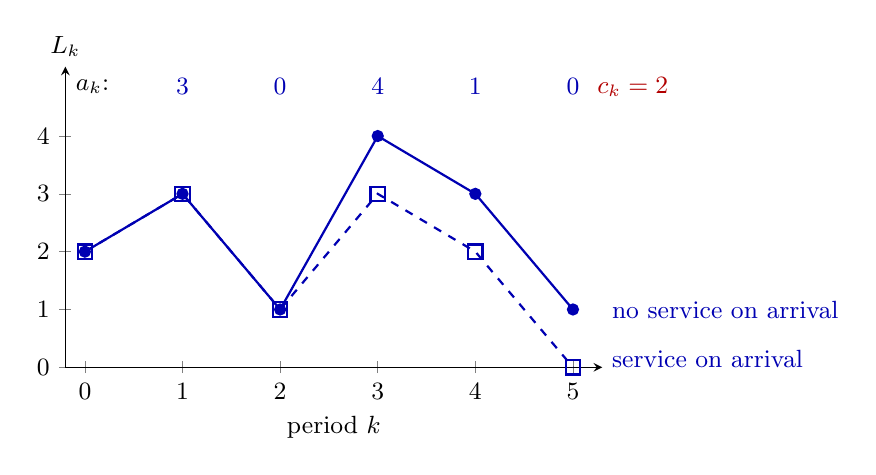
\begin{tikzpicture}[font=\small, >={Latex[length=2mm]}]
  \begin{axis}[
    axis lines=left, xmin=-0.2, xmax=5.3, ymin=0, ymax=5.2,
    xtick={0,1,2,3,4,5}, ytick={0,1,2,3,4},
    xlabel={period $k$}, ylabel={$L_k$},
    xlabel style={at={(axis description cs:0.5,0)}, anchor=north, yshift=-14pt},
    ylabel style={rotate=-90, at={(axis description cs:0,1)}, anchor=south},
    width=8.4cm, height=5.4cm, clip=false
    ]
    \addplot[blue!70!black, thick, mark=*, mark size=1.8pt] coordinates {(0,2) (1,3) (2,1) (3,4) (4,3) (5,1)};
    \addplot[blue!70!black, thick, dashed, mark=square, mark size=2.6pt, mark options={solid}] coordinates {(0,2) (1,3) (2,1) (3,3) (4,2) (5,0)};
    \node[blue!70!black, anchor=west] at (axis cs:5.3,1) {no service on arrival};
    \node[blue!70!black, anchor=west] at (axis cs:5.3,0.15) {service on arrival};
    % arrivals per period
    \node[anchor=east] at (axis cs:0.35,4.85) {$a_k$:};
    \node[blue!70!black] at (axis cs:1,4.85) {$3$};
    \node[blue!70!black] at (axis cs:2,4.85) {$0$};
    \node[blue!70!black] at (axis cs:3,4.85) {$4$};
    \node[blue!70!black] at (axis cs:4,4.85) {$1$};
    \node[blue!70!black] at (axis cs:5,4.85) {$0$};
    \node[red!70!black, anchor=west] at (axis cs:5.15,4.85) {$c_k=2$};
  \end{axis}
\end{tikzpicture}
\end{document}
